%
% Computer Vision - WS2013
% Abgabeprotokoll Exercise 2
%
%
%{{{ misc
\documentclass[subfigure,epsfig,fleqn,float,numbers=noenddot]{scrartcl}

\usepackage{graphicx}
\usepackage{epstopdf}
\usepackage{caption}
\usepackage{subcaption}
\usepackage{amsmath}
\usepackage[T1]{fontenc}
\usepackage[utf8]{inputenc}
\usepackage{amssymb}

\usepackage{pgfplots}

%Zitieren:
\usepackage[english]{babel}
%\usepackage[german]{babel}
\usepackage{babelbib} % f�r das Erstellen des Bibtex-Literaturverzeichnisses
\usepackage{cite}
%\selectbiblanguage{english}
%\selectbiblanguage{german}

%Peseudocode
\usepackage{algpseudocode}
\usepackage{algorithm}

%For Sourcecode
\usepackage{listings}

%Fancy shit
\usepackage{url}

\usepackage[pdftitle={Computer Vision - 2nd Exercise Round},
 						pdfauthor={Matthias Gusenbauer},
						pdfauthor={Robin Melán},
						pdfauthor={David Pfahler},
            pdfsubject={Computer Vision},
            pdfborder={0 0 0}]{hyperref}


\usetikzlibrary{plotmarks}
\pgfplotsset{compat=newest} 
\pgfplotsset{plot coordinates/math parser=false}

%%%%%%%%%%%%%%%%%%%%%%%%%%%%%%%%
% Titlepage

\pagestyle{empty}


%set dimensions of columns, gap between columns, and paragraph indent

\setlength{\textheight}{24.7 cm}
\setlength{\columnsep}{1 cm}
\setlength{\textwidth}{16 cm}
%\setlength{\footheight}{0.0 cm}
\setlength{\topmargin}{0.0 cm}
\setlength{\headheight}{0.0 cm}
\setlength{\headsep}{-0.3 cm}
\setlength{\oddsidemargin}{0.0 cm}
\setlength{\parindent}{0 cm}
\setlength{\parskip}{0.5em}
\setlength{\mathindent}{0mm}

% set page counter if document is part of proceedings
\setcounter{page}{1}
\renewcommand{\floatpagefraction}{0.9}
\renewcommand{\textfraction}{0.1}

% Set the Counters like in the exercise sheet
\setcounter{section}{3}
\renewcommand{\thesection}{Assignment \arabic{section}:}
\renewcommand{\thesubsection}{\Alph{subsection}.}

%\renewcommand{\captionlabelfont}{\fontfamily{phv}\fontseries{bx}\fontsize{10}{10pt}\selectfont}
%\renewcommand{\captionfont}{\fontfamily{phv}\fontsize{10}{12pt}\selectfont}
%\setlength{\captionmargin}{0.5 cm}

\makeatletter
\makeatother
\def\RR{\hbox{I\kern-.2em\hbox{R}}}

\begin{document}

%don't want date printed
\date{\today}

%make title bold and 14 pt font (Latex default is non-bold, 16pt) 
\title{~\\
	\fontsize{12}{12pt} \bf Computer Vision 183.585 VU 3.0 4.5 ECTS
  ~\\[0.7cm]
  \fontsize{14}{14pt} \bf 2nd Exercise Round}
  

%for single author 
\author{~\\
  ~\\
  \fontsize{12}{12pt}
  {\bf David Pfahler, Matthias Gusenbauer, Robin Melán}\\
  1126287, 1125577, 1029201
  ~\\ ~\\ ~\\
  \normalsize
}

\maketitle
%I don't know why I have to reset thispagestyle, but otherwise get page numbers 
\normalfont
\thispagestyle{empty}

%%%%%%%%%%%%%%%%%%%%%%%%%%%%%%%%%%%%%%%%%%%%%%%%%%%%%%%%%%%%%%%%%%%%%%%%%%%%%%%%
% CONTENT

\section{Image Stitching}
\label{sec:1}

\subsection{SIFT Interest Point Detection}
\label{sec:A}
As the first part of the assignment we need to extract SIFT features out of every image separately.\footnote{See Matlab-file \emph{GetSIFTFeatures.m} } Therefore we convert the image to \emph{rgb2gray(image)} and method $[text{key, desc}] = vl\_sift(siftIm);$ to extract the features from our image. The \emph{key} value consists of a 4 x n matrix, where n is the number of features found in the image, holding the x-coord., y-coord., the scale (s) factor and the orientation (in radiant). The $desc$ value holds an 128 dimensional vector for every $key$, which describe the eigenvectors (See Example in Figure \ref{img:sift}). 
	\begin{figure}[H]
		\centering
		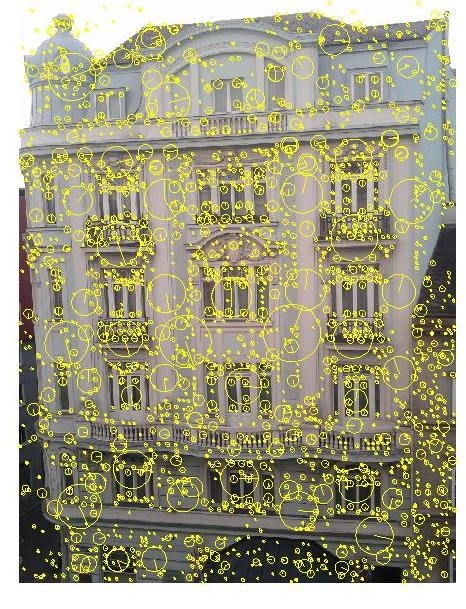
\includegraphics[width=0.55\textwidth]{./img/siftDesc2.jpg}
		\caption{Extracted Sift Features}
		\label{img:sift}
	\end{figure}

\subsection{Interest Point Matching and Image Registration}
\label{sec:B}
The next step consists of determining the homographies between all image pairs from left to right. So we start of with computing the first homography $H_\text{1,2}$ and continue until homography $H_\text{5,4}$ (I switch 5 and 4 because I need to transform the 5th image into the 4th, if I am taking the image in the middle as reference, see further \ref{sec:C}).\footnote{See Matlab-file \emph{IntPointMatching.m} } \\
To compute the homography we first need to follow a couple of steps, starting by matching our descriptors $[matches, scores] = vl\_ubcmatch(descriptor1, descriptor2);$. $Matches$ contains the indices of the original (first) and closest descriptor in the other (second) image. The $scores$ value holds the euclidean distance between them.\\
	\begin{figure}[H]
		\centering
		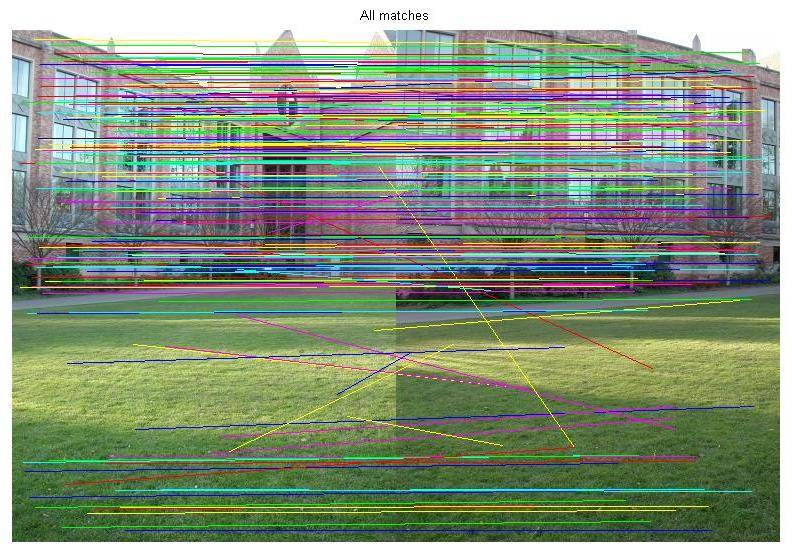
\includegraphics[width=0.85\textwidth]{./img/allMatches.jpg}
		\caption{All the Matches that where found between the two Images, as we can see some of them are outliers - therefore we need the RANSAC scheme to get rid of them, so we don't get a distorted homography at the end.}
		\label{img:outliers}
	\end{figure}
As we can see in Figure \ref{img:outliers} not all of our found matches are essentially correct, some of them are considered to be $outliers$ and if we would compute a homography including them we would get a distorted result. Therefore we apply the RANSAC scheme to receive a better estimation of the homography between the image pair.\footnote{See Matlab-file \emph{PerfRANSAC.m} } 
\par We begin by selecting randomly 4 matched-points pairwise (see Figure \ref{img:points} ) and estimate the homography between them by using the given function $cp2tform()$ as follows.
\begin{lstlisting}
$[homography] = cp2tform(rndPnts1, rndPnts2, 'projective')$. 
\end{lstlisting}
After acquiring the homography we transform all found points of interest and measure how many points are below a given threshold distance $T$ using the euclidean distance as distance metric. This is done in the function tformAInliers() in starting at line 55 in the code below. If the number of inliers in the current iteration of the algorithm is greater than the previous best result then the best homography gets updated to the current one. After $N$ iterations the inliers of the best matching homography are used to reestimate the homography which is then used to transform the image in step $C)$. 

\begin{lstlisting}[language=Matlab, numbers=left, numberstyle=\tiny]
function [ homography ] = PerfRANSAC( points1, points2 ,image1, image2, doPlot)

N = 1000;
bestInliersCnt = 0;
bestInliers = 0; 
bestHomo = 0;


for(i=1:N)
    randoms = randsample(size(points1, 1),4);
    
    rndPnts1 = points1(randoms,:);
    rndPnts2 = points2(randoms,:);
        
    try
        % b) - d)
        [nrInliers, inliers, TFORM] = tformAInliers(points1, points2, rndPnts1, rndPnts2);
        
        % if new calculation is better than old update result
        if(nrInliers > bestInliersCnt)
            disp(sprintf('Best match - #of inliers \%d', nrInliers));
            bestInliersCnt = nrInliers;
            bestInliers = inliers; 
            bestHomo = TFORM;
        end
        
    catch err
        disp('Ouch!');
    end
end

% 4) after N runs take best homography and reestimate with all points
% saving only the inliners from points1 and 2
m1 = zeros(bestInliersCnt,2);
m2 = zeros(bestInliersCnt,2);

pos = 1;
for i = 1:size(bestInliers,1)
    if (bestInliers(i) == 1)
        m1(pos,:) = points1(i,:);
        m2(pos,:) = points2(i,:);
        pos = pos + 1;
    end
end

% Output all inliers:
if (doPlot)
    match_plot(im2double(image1{1,1}), im2double(image2{1,1}), m1, m2);
    title('Matches of only Inliers!');
end
[~, ~, homography] = tformAInliers(points1, points2, m1, m2);

end

function [ nrInliers, inliers, homography ] = tformAInliers( points1, points2, rndPnts1, rndPnts2)

T = 5;

% b) estimate transformation ob rndPnts1 onto rndPnts2
homography = cp2tform(rndPnts1, rndPnts2, 'projective');

% c) transform the points 
trnsfrmdPnts = tformfwd(homography, points1(:,1), points1(:,2));

% d) calc euclidean distance
distance = (trnsfrmdPnts - points2).^2; %one line sqrt(sum(.))
distance = sqrt(distance(:, 1) + distance(:, 2));

% Thresholding
inliers = distance<=T;
nrInliers = sum(inliers);

end
\end{lstlisting}

	\begin{figure}[H]
		\centering
		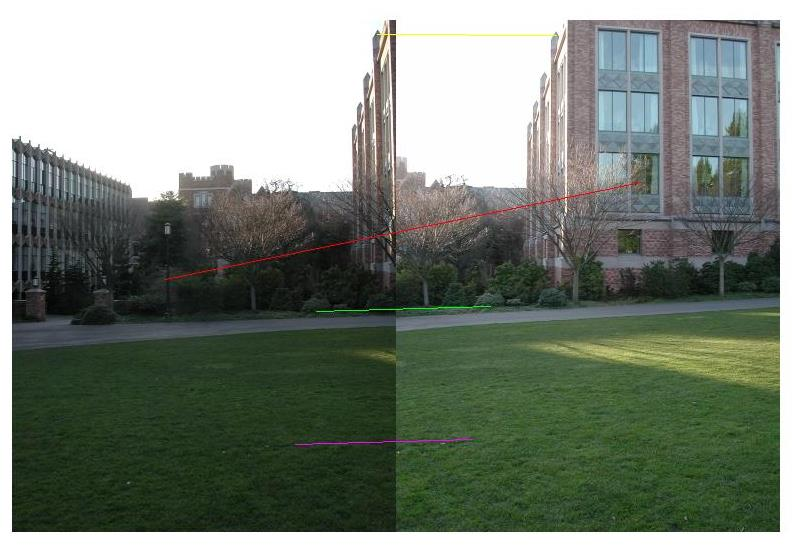
\includegraphics[width=0.55\textwidth]{./img/fourRandomMatches.jpg}
		\caption{Select randomly 4 matched-points}
		\label{img:points}
	\end{figure}

\subsection{Image Stitching}
\label{sec:C}
So after we determined the homographies between all the image pairs we select the image in the middle (in our case Image 3) to be our reference image and compute all homographies that map the other images to our reference:
\begin{equation*}
\\H_{1,3} = H_{2,3} * H_{1,2} \\
H_{5,3} = H_{4,3} * H_{5,4} 
\end{equation*}
Before we can stitch our images into one panorama picture we need to compute the size the output image is going to have. For this information we can take the method $imtransform$ with our new homographies and as a result we get the new size (xData, yData) of the transformed image, which is saved in our case for all 4 images (we don't need to compute the reference image, because we know it is going to be in the middle of the panorama picture) in an array: 
\begin{lstlisting}[language=Matlab, numbers=left, numberstyle=\tiny]
%% saves the dimensions of all the transformed images
xLim = zeros(4,2);
yLim = zeros(4,2);
	
[transImage, xLim(1,:), yLim(1,:)] = imtransform(Images{1}, H_1_3);
...
	
%% Getting the Coordinates for final Image
xMin = min(min(xLim));
xMax = max(max(xLim));
   
yMin = min(min(yLim));
yMax = max(max(yLim));
   
%% Width and Height of panorama image.
width  = round(xMax - xMin);	
height = round(yMax - yMin);
\end{lstlisting}

Now that we know the output dimensions of our final panorama image we can transform all of our images into that particular size by using again the $imtransform$ method but this time adding our appropriate dimensions [xMin xMax] and [yMin yMax] as our XData and YData parameters. Given all transformed images, the final step is to blend them together in a way to avoid seams. To do this we use an $\alpha$ channel where the value of $\alpha$ for an image is 0 at all border pixels and 1 at the maximum distance from the border. The remaining values are linearly interpolated (see Figure \ref{img:bwdist}) and transformed with their respective homography to the panoramic image. For Example our interpolation value $\alpha$ would look like Figure \ref{img:interpolation} for all our 5 images. The final color at a pixel in the output image is computed as the $\alpha$-weighted sum of overlapping images. More precisely, if there are $n$ images overlapping at pixel position $(x,y), I_i(x,y), i = 1...n$ with color $(R_i,G_i,B_i)$ and weighting factors $\alpha_i$, the color values in the stitched output image O are computed as follows:
\begin{equation*}
	O(x,y) = \frac{\sideset{}{_{i=1}^n}\sum_{} (R_i,G_i,B_i) * \alpha_i} {\sideset{}{_{i=1}^n}\sum_{} \alpha_i}
\end{equation*}

This blending method is called $feathering$.
	\begin{figure}[H]
		\centering
		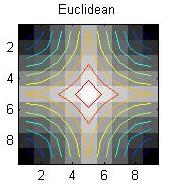
\includegraphics[width=0.65\textwidth]{./img/bwdist.jpg}
		\caption{To compute our $\alpha$ channel we used the method $bwdist$ with the euclidean distance method}
		\label{img:bwdist}
	\end{figure}
	\begin{figure}[H]
		\centering
		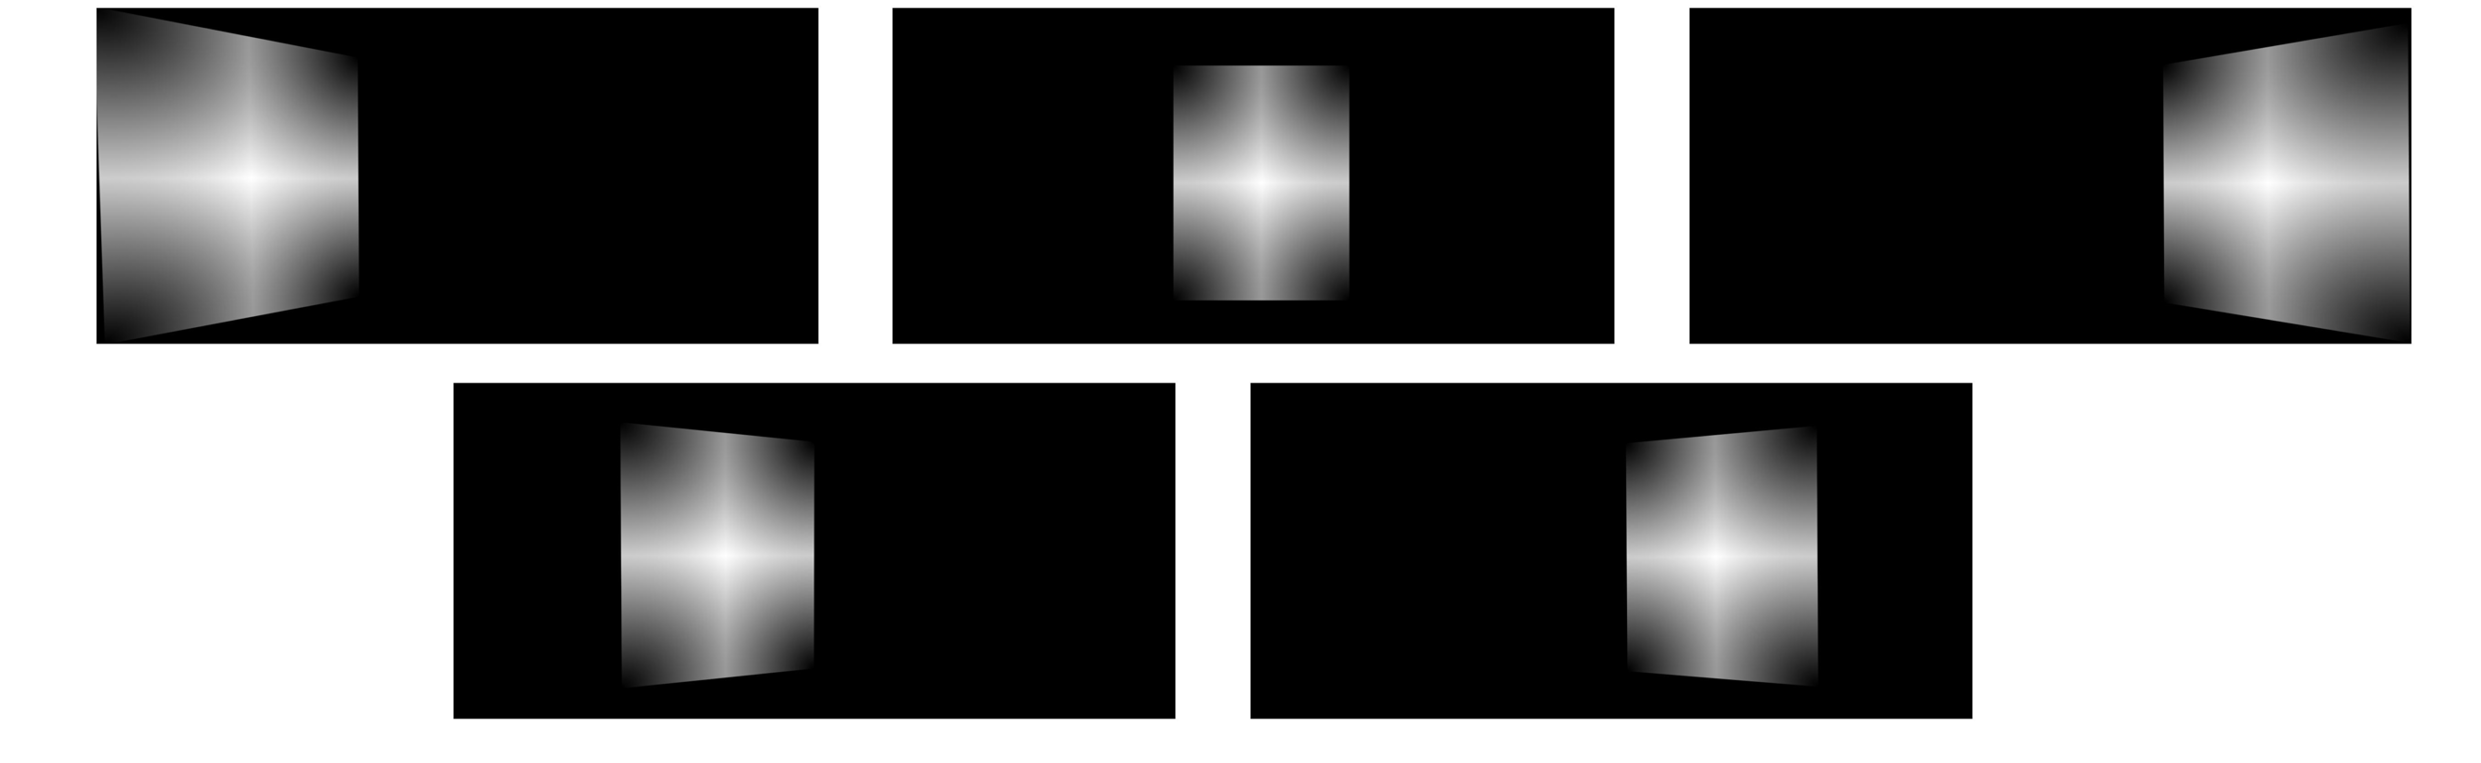
\includegraphics[width=0.95\textwidth]{./img/interpolationImg.png}
		\caption{$\alpha$ channel the interpolation of the 5 images to the resulting panorama picture}
		\label{img:interpolation}
	\end{figure}
	
\paragraph{Results}
Our first set of images $campus1...5.jpg$ with $feathering$:
\begin{figure}[H]
		\centering
		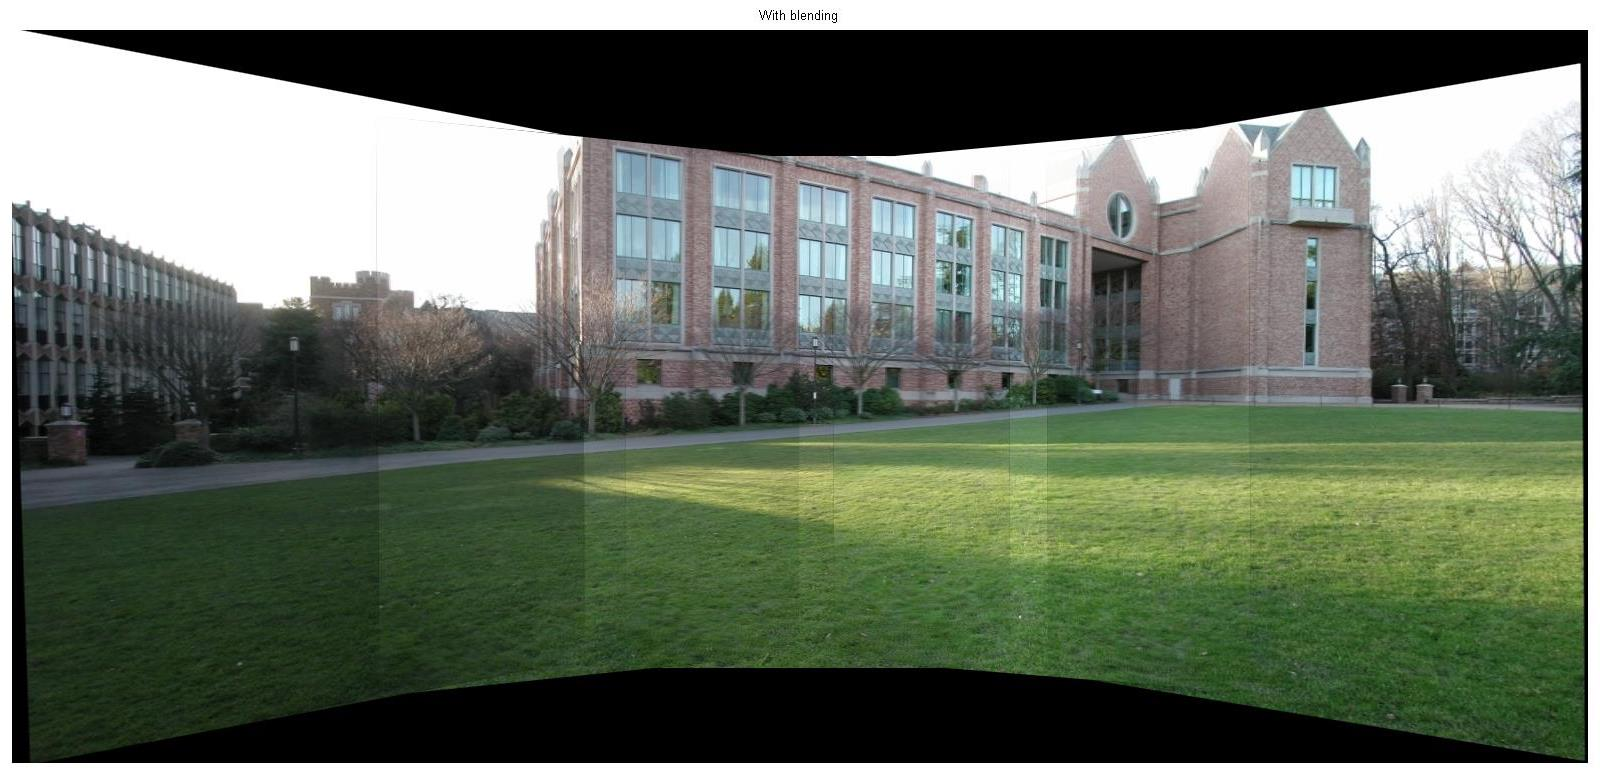
\includegraphics[width=0.95\textwidth]{./img/withBlending.jpg}
		\caption{Sample Set campus\{1...5\} with feathering}
		\label{img:withBlend}
\end{figure}
And without $feathering$ (the transformed images are laid over each other from left to right):
\begin{figure}[H]
		\centering
		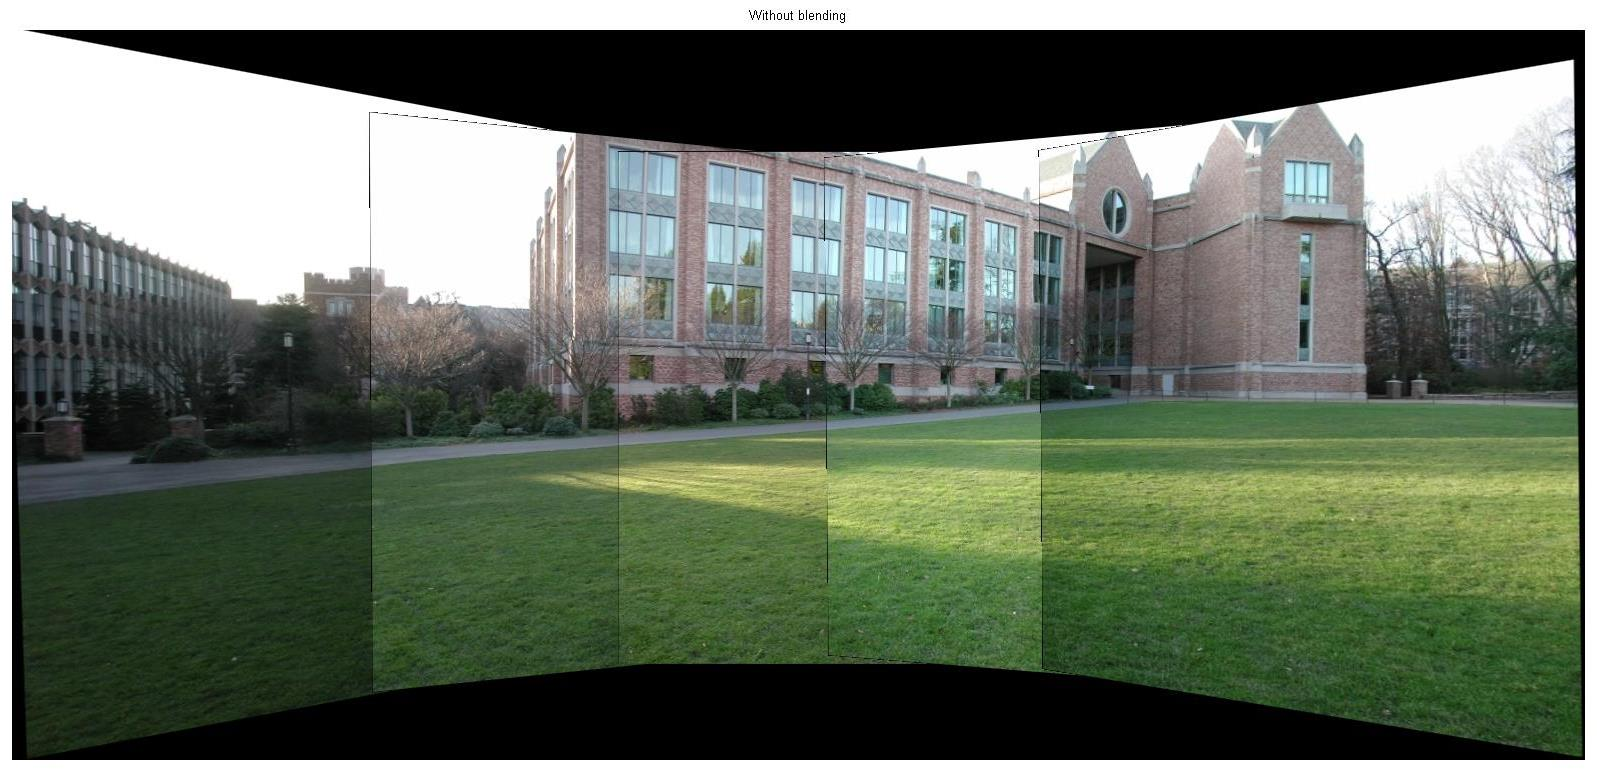
\includegraphics[width=0.95\textwidth]{./img/withoutBlending.jpg}
		\caption{Sample Set officeview\{1...5\} with feathering}
		\label{img:withoutBlend}
\end{figure} 
Our second set of images $officeview1...5.jpg$ with $feathering$:
\begin{figure}[H]
		\centering
		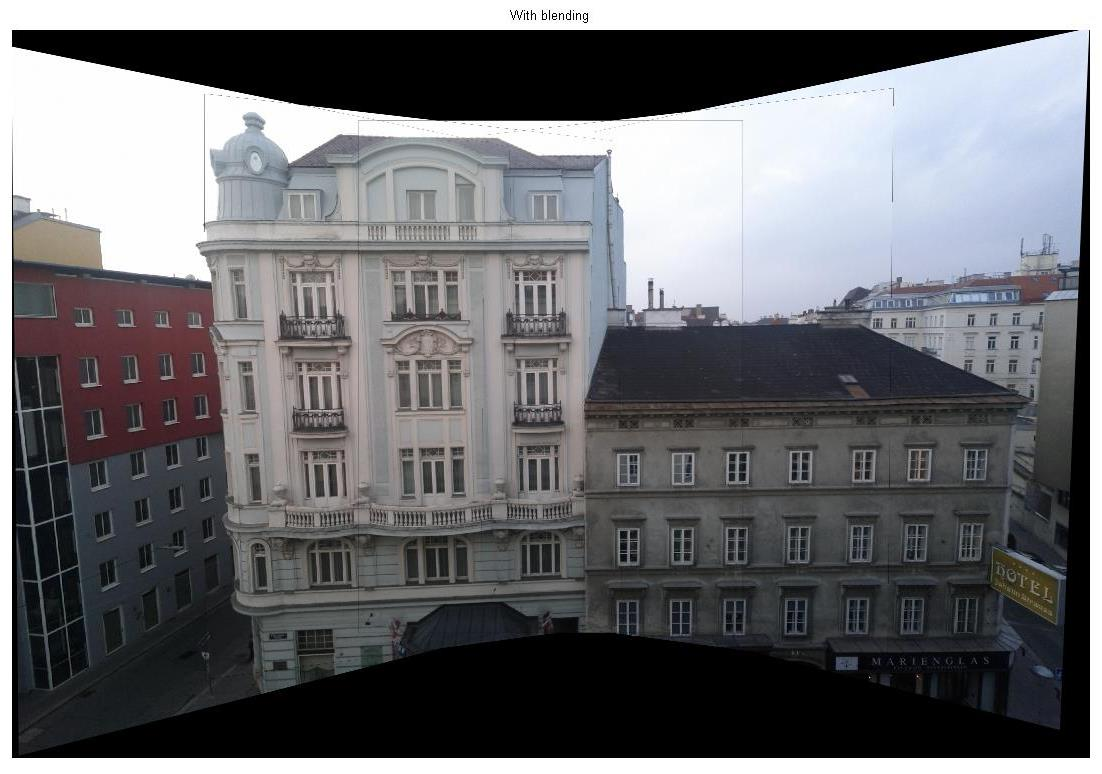
\includegraphics[width=0.95\textwidth]{./img/withBlending2.jpg}
		\caption{Sample Set officeview\{1...5\} with feathering}
		\label{img:withBlend2}
\end{figure}
And without $feathering$ (the transformed images are laid over each other from left to right):
\begin{figure}[H]
		\centering
		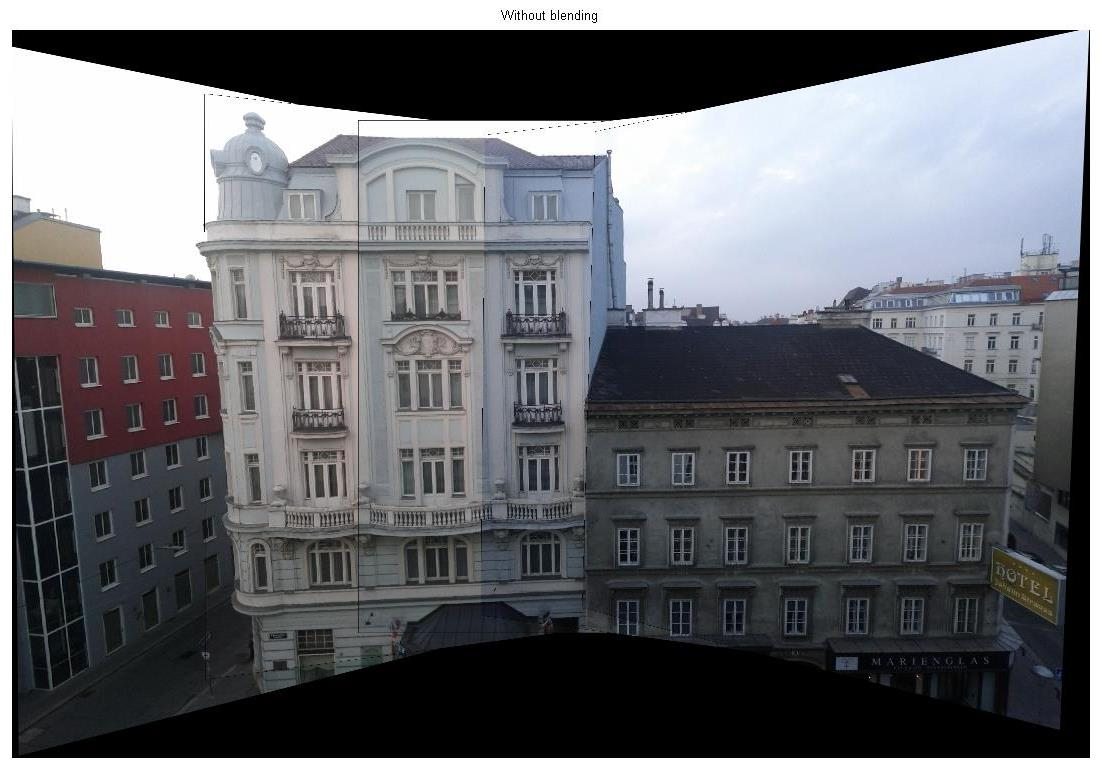
\includegraphics[width=0.95\textwidth]{./img/withoutBlending2.jpg}
		\caption{Sample Set campus\{1...5\} with feathering}
		\label{img:withoutBlend2}
\end{figure}

\begin{figure}[H]
		\centering
		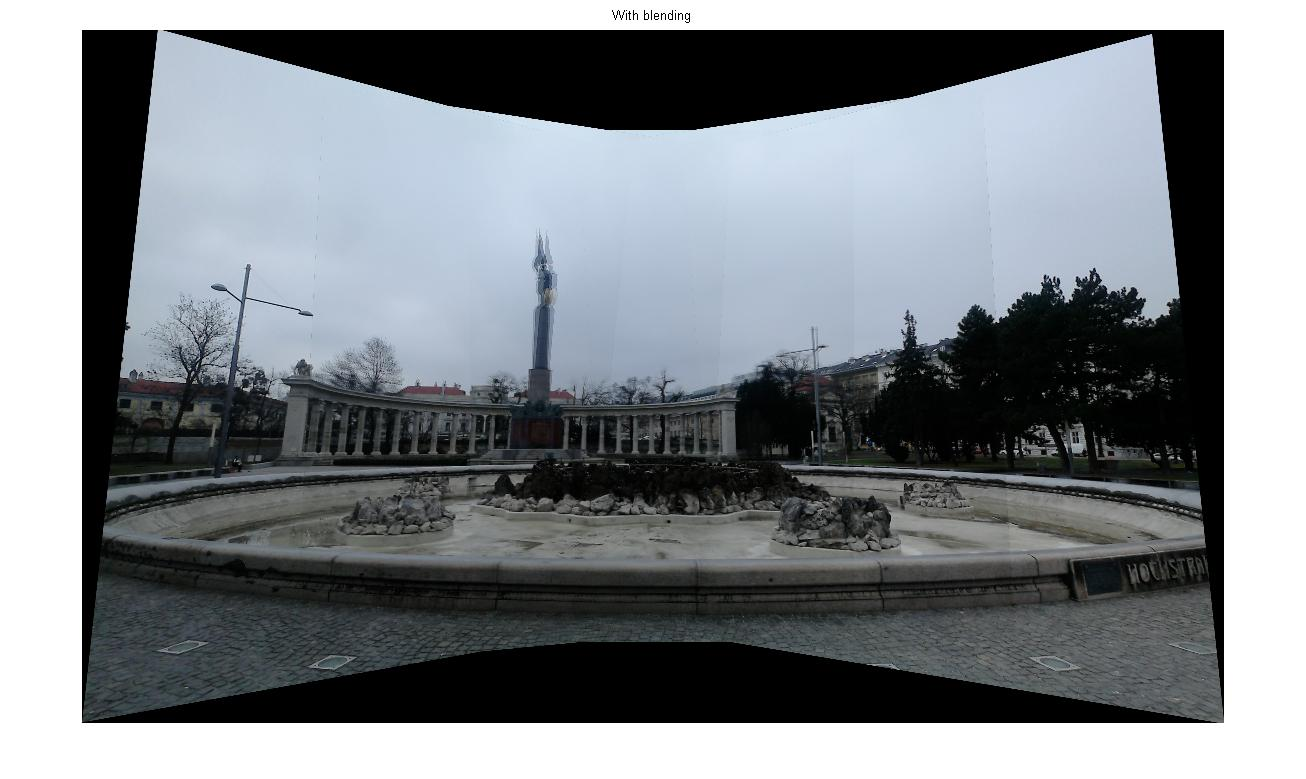
\includegraphics[width=0.95\textwidth]{./img/soldier.jpg}
		\caption{Sample Set campus\{1...5\} with feathering}
		\label{img:own1}
\end{figure}

\begin{figure}[H]
		\centering
		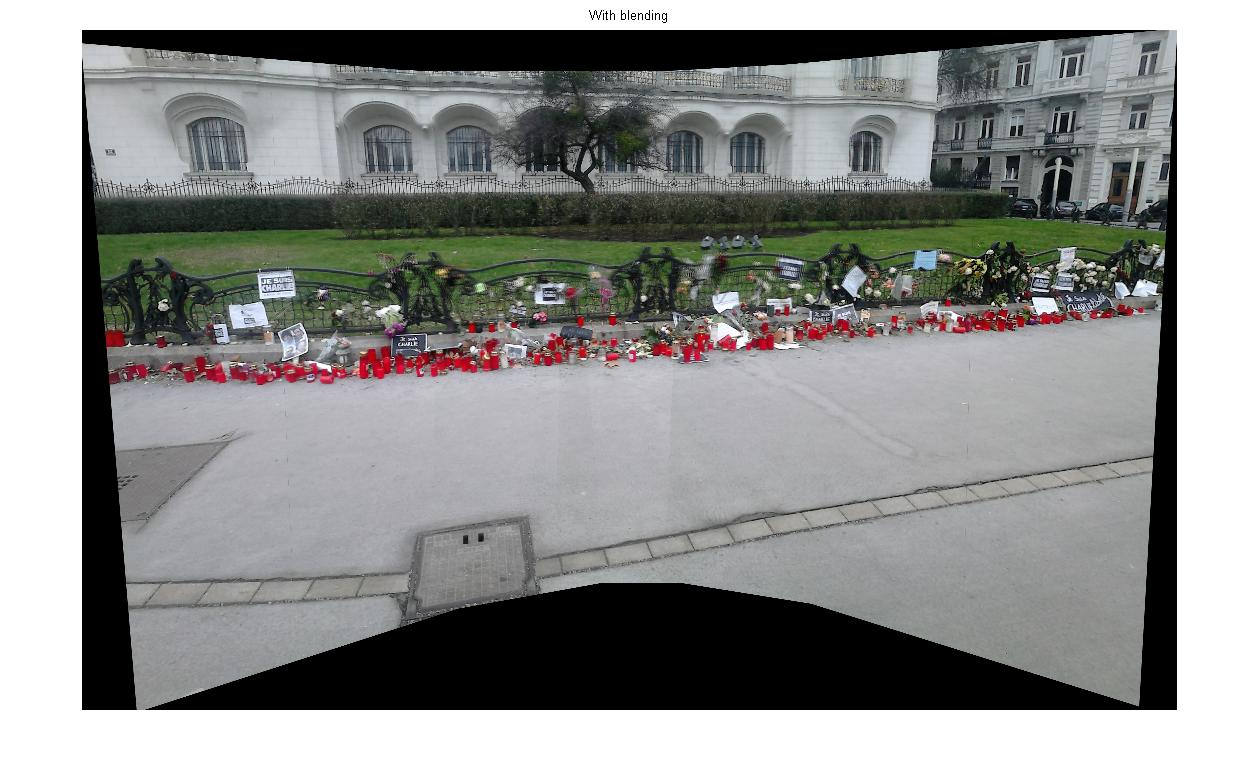
\includegraphics[width=0.95\textwidth]{./img/charlie.jpg}
		\caption{Sample Set campus\{1...5\} with feathering}
		\label{img:own2}
\end{figure}

Especially looking at the first and the first self-made image (see Figure \ref{img:withBlend} \ref{img:own1}) we see that some of the images could not be overlaid correctly, which means that there still were some small outliers which distorted the homography so that the final image is at some parts a little blurry. 
With the second sample and the self-made images (see Figure \ref{img:withBlend2} \ref{img:own1} \ref{img:own2}) we detect the $feathering$ effect much better than for the first image because the shading through the image is continuous and no seams are visible from overlapping one image after another. 


\section{Scene Recognition with Bag of Visual Words}
\label{sec:2}

In this assignment we want to classify images into scene categories like bedroom, kitchen etc. 
We use the standard bag of visual words model to achieve this task. Subsection~\ref{sec:methodology} presents the implementation of the category recognition and Subsection~\ref{sec:results} presents our results.

\subsection{Methodology}
\label{sec:methodology}

First the test- and the training-set gets loaded and for every image its category is saved. The next step is to build a vocabulary
of visual words. We will form this vocabulary by sampling many local features from our training set and then clustering them with K-means. The number of K-means clusters \texttt{num\_clusters} is the size of our vocabulary. We used 50 clusters which means that the 128 dimensional SIFT feature space is partitioned into 50 regions.\\
Every time a new SIFT feature gets observed, the cluster it belongs to can easily get figured out by getting the nearest centroid of our original clusters. Those clusters are our visual word vocabulary.\\
To extract these SIFT features from the images in the training set to collect them for k-means clustering, 100 SIFT features get extracted from every image. These features get added to the feature space which is $128 \times \mbox{size of training set}*\mbox{number of features per image}$. In out example the training set contains 800 images and the number of features per image is also 100, that means the feature space is $128 \times 80000$ big. After that the 50 clusters get determined and stored in a matrix.\\
The next step is to build a feature representation for every image in the training set that can be used for the classification of new images later on. An image is represented by the normalized histogram of visual words, which means that all SIFT features of an image are assigned to visual words and the number of occurrences of every word is counted. Therefor we have to get the SIFT features for every image from the training set again, but this time it gets sampled more densely than before. We used a step size of 2. Then we determine the nearest clusters of the sampled SIFT-features and count the number of occurrences. This histogram represents the bag of words for this image.\\
The last step is to classify all the images of the test set to investigate the classification power of the bag of visual words model for our classification task. This is obviously quite similar to the previous step. (Get SIFT features densely sampled (step size is 2) and count number of nearest clusters to this features as bag of words) But this time the visual word histogram of an image is used for actual classifying it by means with the nearest neighbor method (we used a k of 3) with the previously learned training features and class labels. The result is stored in a confusion matrix. (See Figure~\ref{fig:conf_matrix_test})

\subsection{Results}
\label{sec:results}

\paragraph{Classification Rate}
\label{sec:classification}
Figure~\ref{fig:conf_matrix_test} shows the classification results of the given test set in form of a confusion matrix. A cell in this matrix describes how many of the test images of the category of the row (e.g. the first row is the category 'bedroom') got classified as the category of the column. For example 92\% of the test images of forests got classified as forests.\\
In general our scene classification results are all higher than 35\% which is really bad. But this is only the case because pictures of bedrooms and living rooms are very similar and it is really hard to distinguish them. Figure~\ref{fig:hardimages} shows two pictures (one living room and one bedroom) which contain many similarities. For example both rooms contain: Lamps, a television, a bed/ a sofa, windows and other furniture.\\
Also pictures of kitchens got confused as livingrooms (16\%) and offices (13\%). And stores got wrongly detected as livingrooms (21\%) and streets (9\%).
Figure~\ref{fig:easyimages} shows that in contrast it is very easy to distinguish between a living room and a forest or a mountain, because nearly no features appear in both images. Only through the windows of the rooms or pictures on the walls it is possible to see nature in human environments. This is also reflected in the classification rate of the forest images which is at 92\%.
We

\paragraph{Own Test Images}
\label{sec:owntestimages}
Figure~\ref{fig:ownimages} shows our own test images. We took 5 images from 5 different categories and tried to categorized them with our scene recognizer. Figure~\ref{fig:conf_matrix_own} shows the results of the scene recognition. As you can see only the picture of the bedroom and of the forest could get recognized correctly, the other 3 images were recognized wrong as bedroom.\\ This is also consistent with the above findings.

\paragraph{Step Size} we also tried to categorize the pictures with a step size of 1, which means the double amount of SIFT features per image. Figure~\ref{fig:stepsize} shows that the results were worse than with the step size of 2. 

\begin{figure}
        \centering
        \begin{subfigure}[b]{0.3\textwidth}
                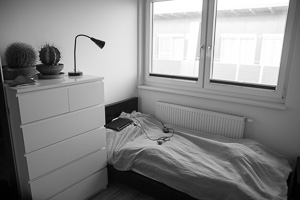
\includegraphics[width=\textwidth]{img/own/bedroom}
                \caption{Bedroom}
                \label{fig:bedroom}
        \end{subfigure}%
        ~
        \begin{subfigure}[b]{0.3\textwidth}
                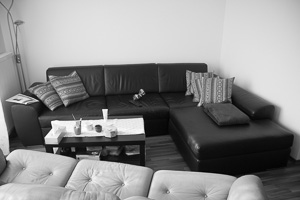
\includegraphics[width=\textwidth]{img/own/livingroom}
                \caption{Livingroom}
                \label{fig:livingroom}
        \end{subfigure}
        ~
        \begin{subfigure}[b]{0.3\textwidth}
                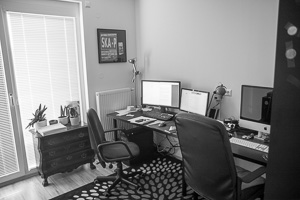
\includegraphics[width=\textwidth]{img/own/office}
                \caption{Office}
                \label{fig:office}
        \end{subfigure}
				
				\begin{subfigure}[b]{0.3\textwidth}
                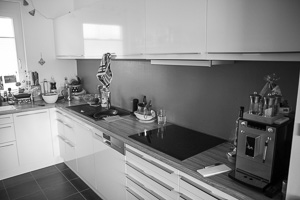
\includegraphics[width=\textwidth]{img/own/kitchen}
                \caption{Kitchen}
                \label{fig:kitchen}
        \end{subfigure}
				~
				\begin{subfigure}[b]{0.3\textwidth}
                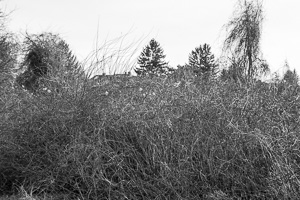
\includegraphics[width=\textwidth]{img/own/forest}
                \caption{Forest}
                \label{fig:forest}
        \end{subfigure}
        \caption{Own scene pictures}\label{fig:ownimages}
\end{figure}

\begin{figure}
		\centering
		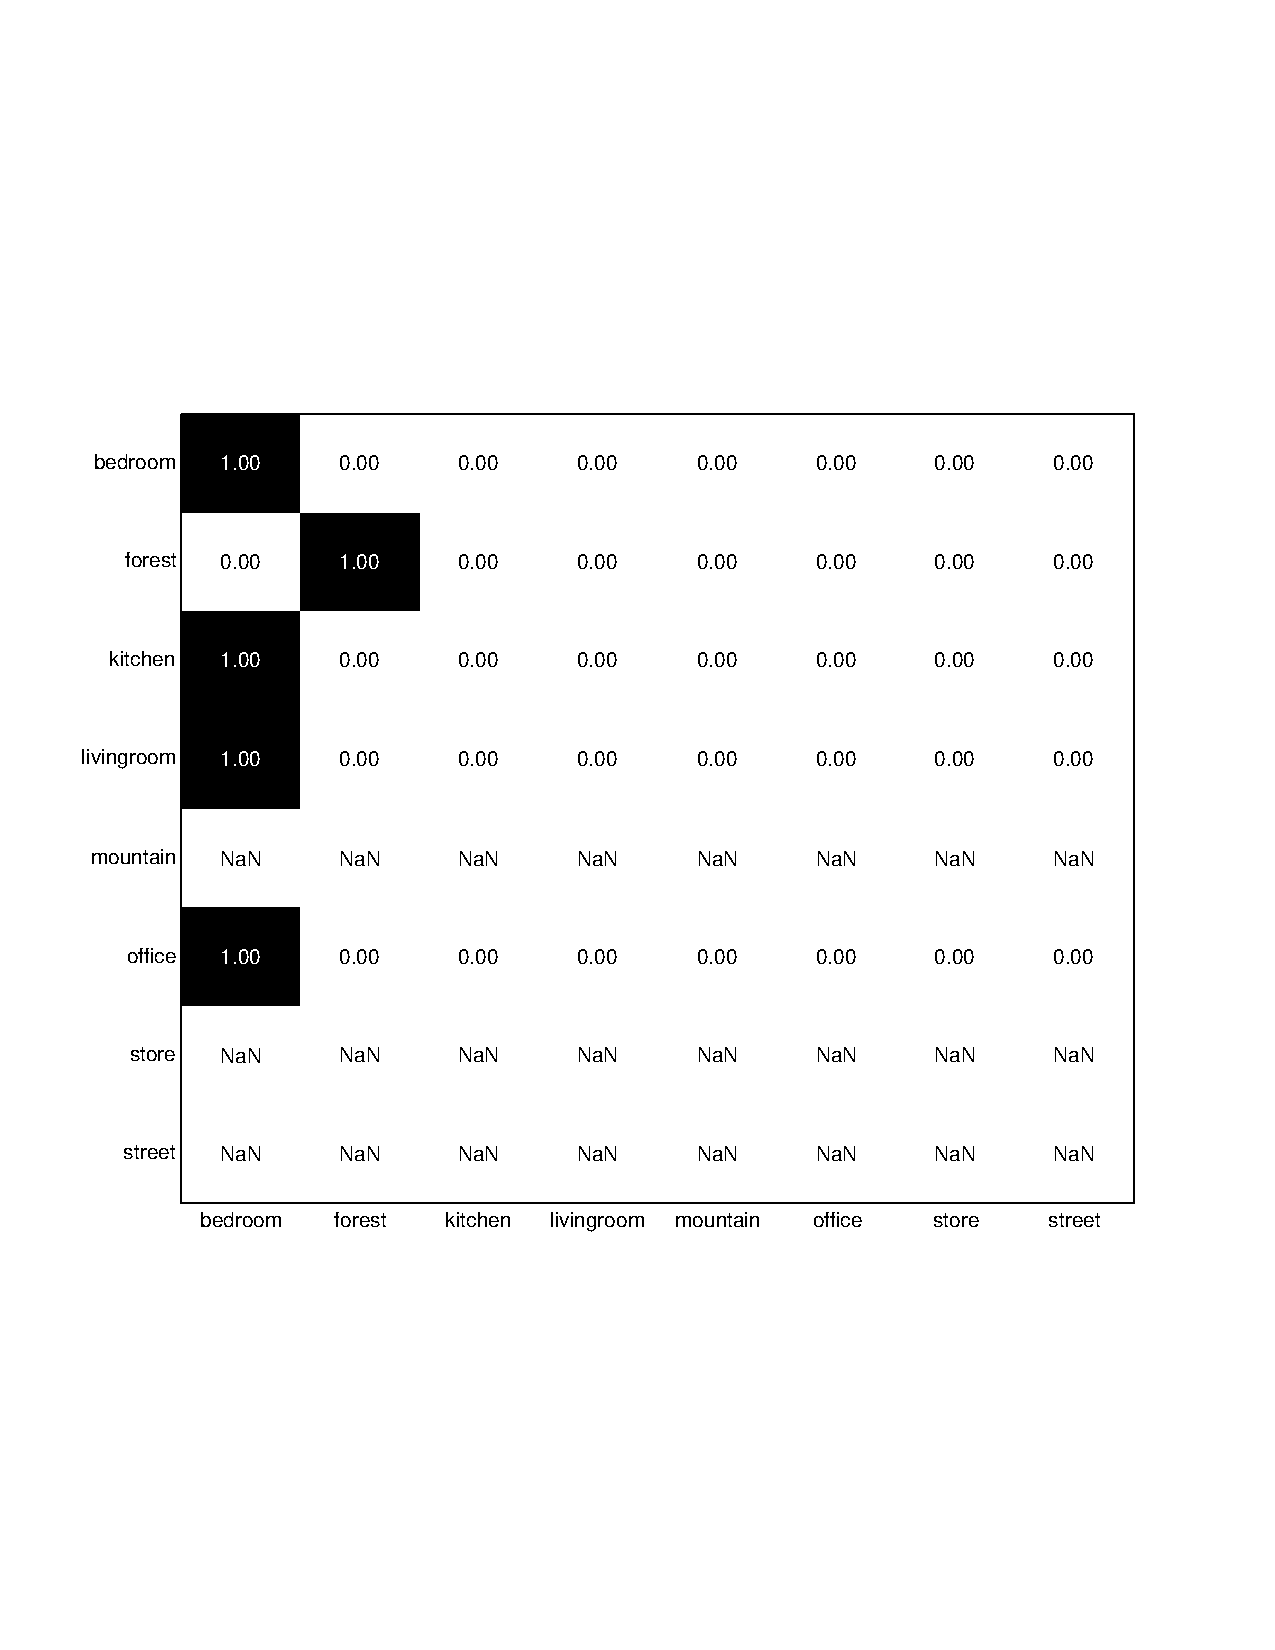
\includegraphics[width=\textwidth]{img/conf_matrix_own.pdf}
		\caption{classification results in percentage of the own pictures in form of a confusion matrix}
		\label{fig:conf_matrix_own}
\end{figure}
\begin{figure}
		\centering
		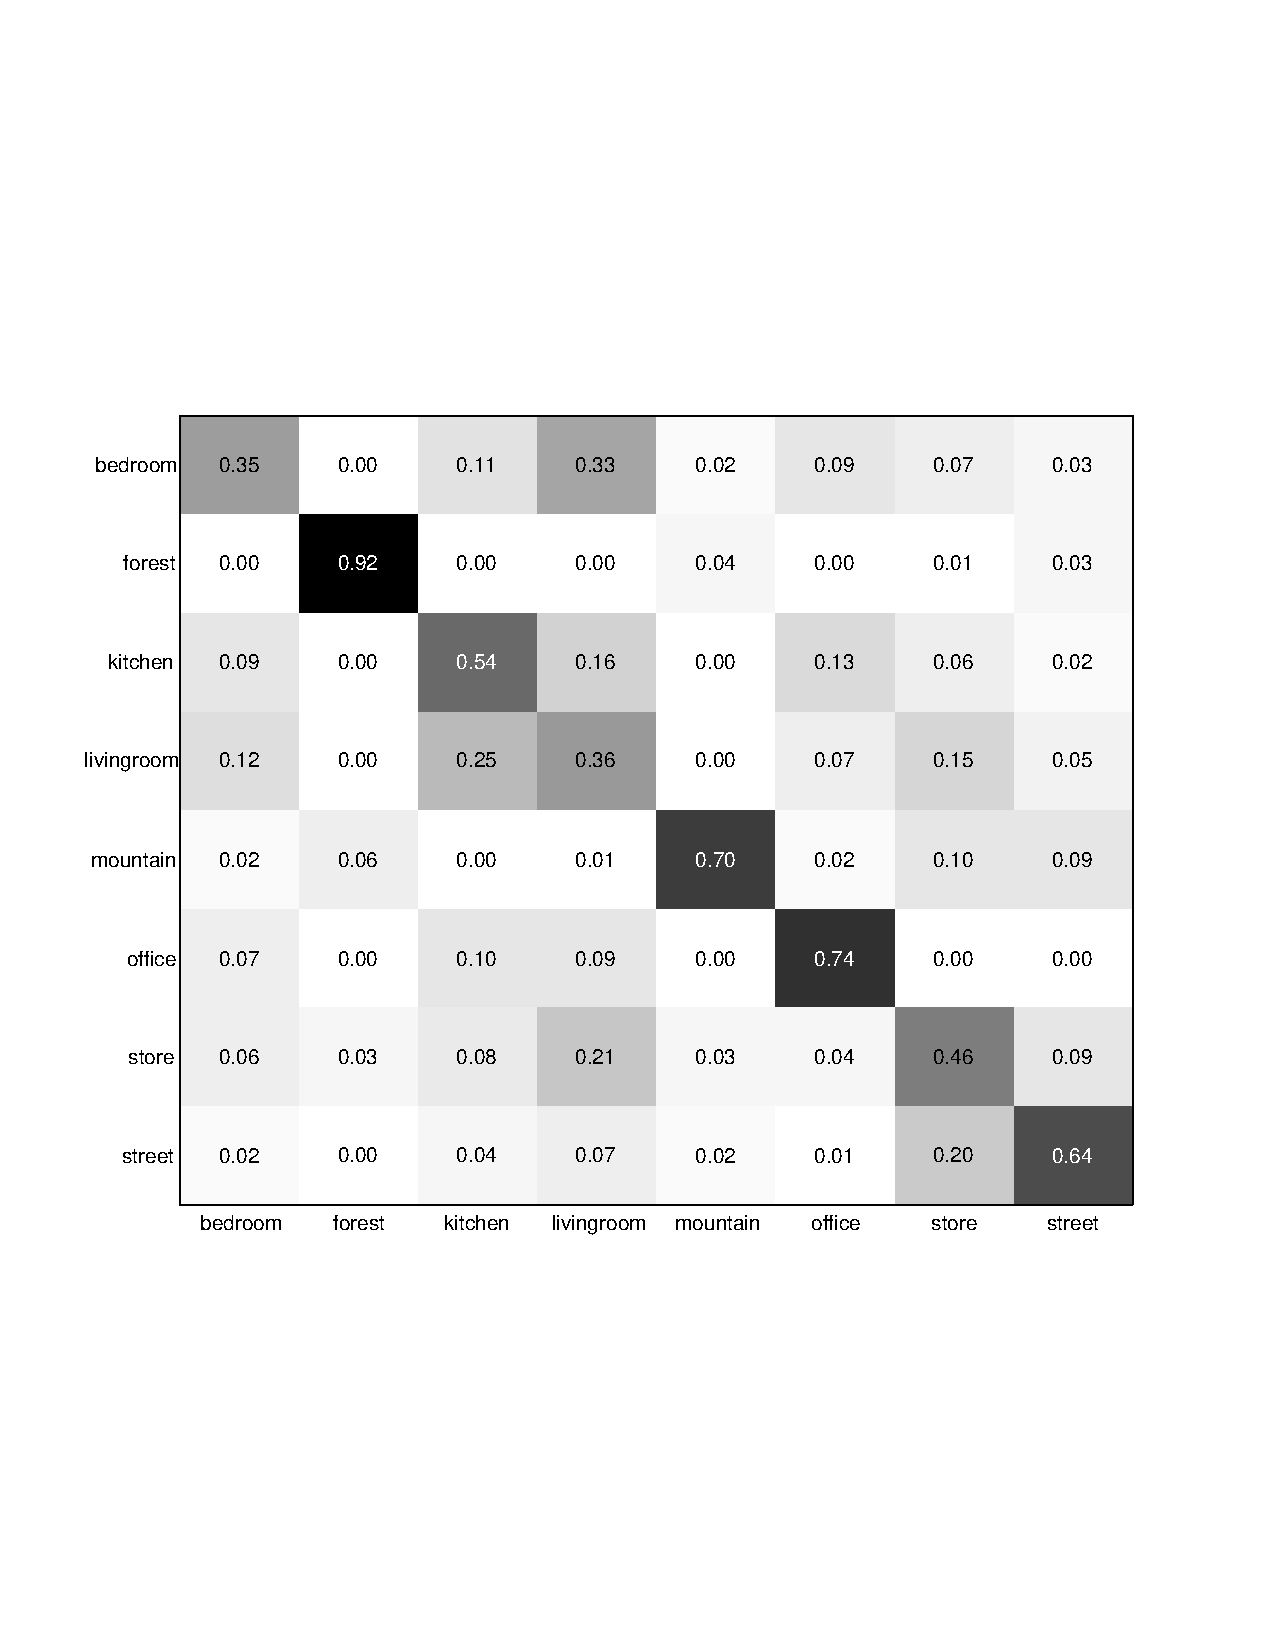
\includegraphics[width=\textwidth]{img/conf_matrix_test.pdf}
		\caption{classification results in percentage of the given test set in form of a confusion matrix}
		\label{fig:conf_matrix_test}
\end{figure}


\begin{figure}
		\centering
		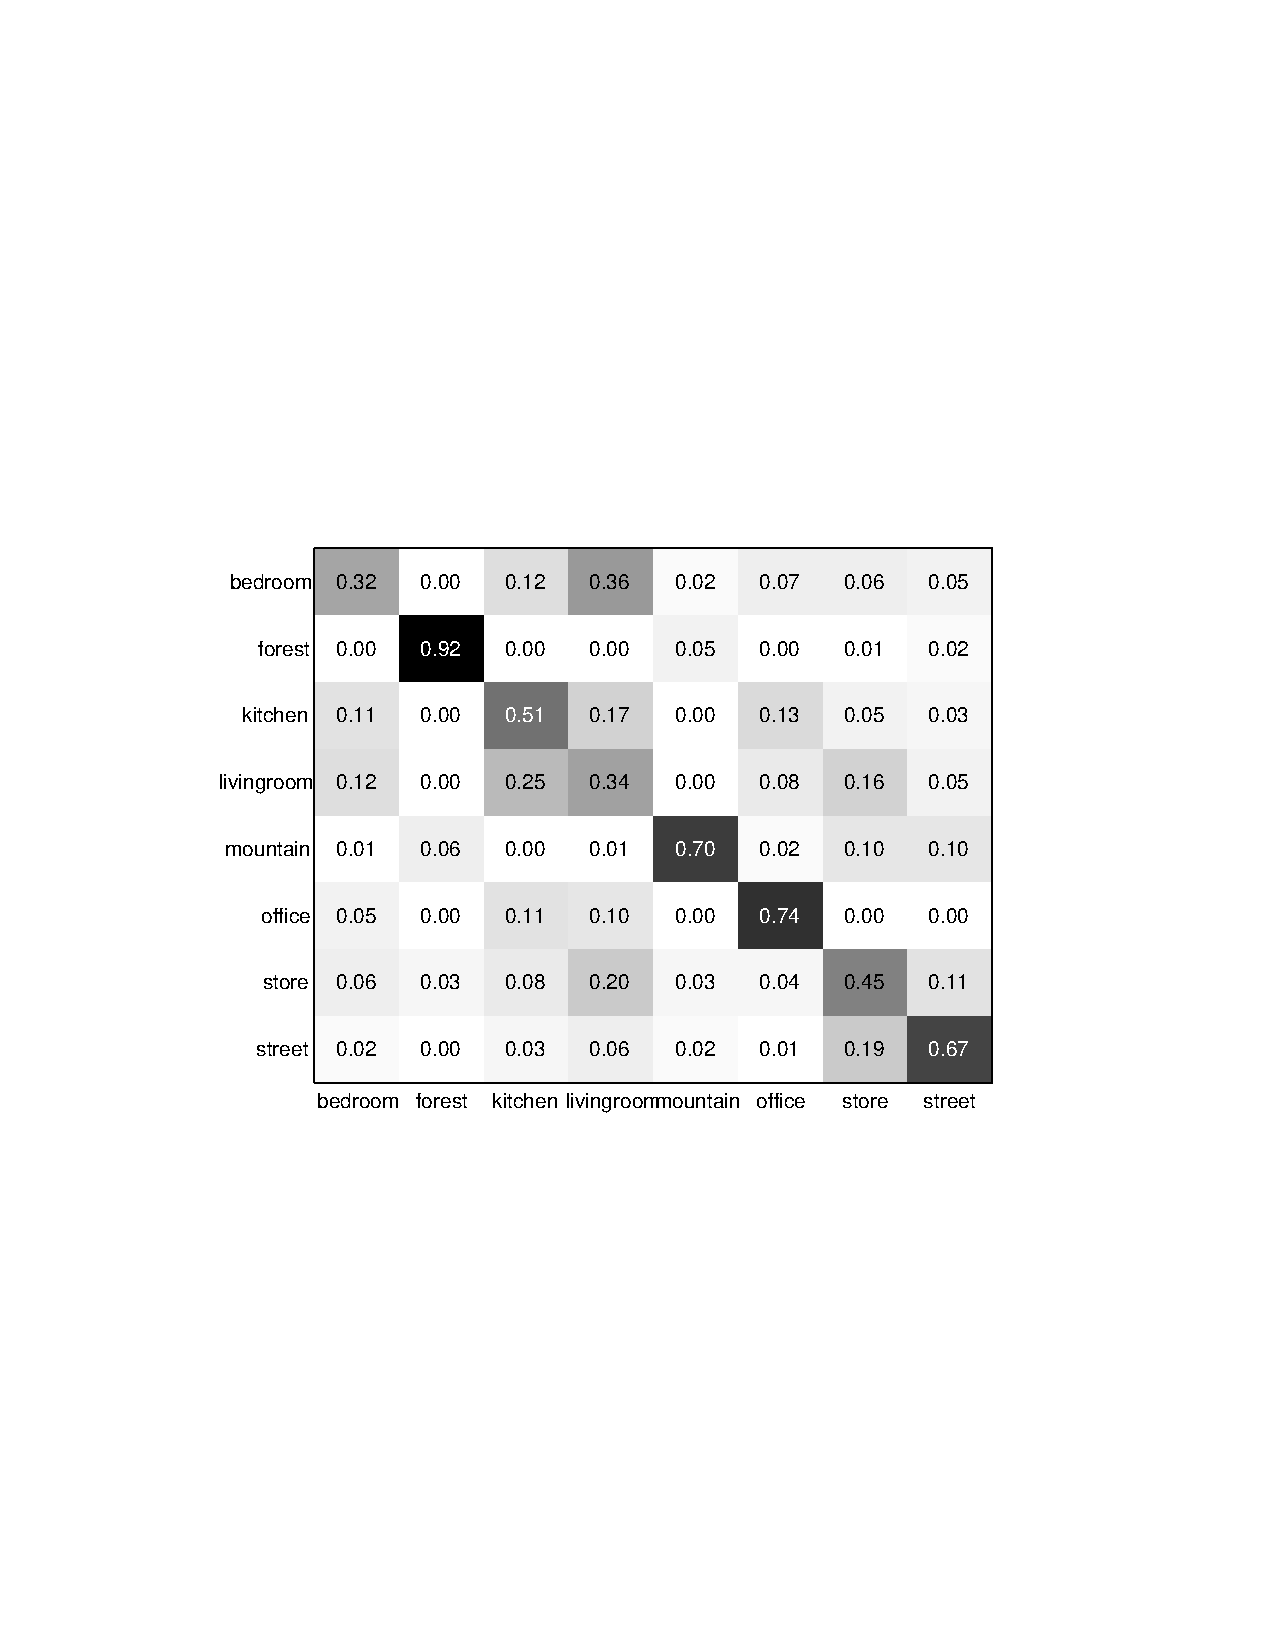
\includegraphics[width=\textwidth]{img/conf_matrix_step1.pdf}
		\caption{classification results in percentage of the given test set in form of a confusion matrix with step size = 1}
		\label{fig:stepsize}
\end{figure}

\begin{figure}%
	\centering
	\begin{subfigure}[b]{0.4\textwidth}
					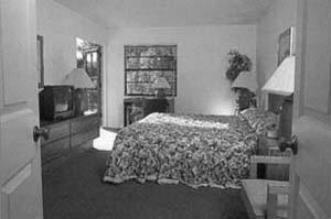
\includegraphics[width=\textwidth]{img/bedroom_hard}
					\caption{Bedroom}
					\label{fig:bedroomhad}
	\end{subfigure}%
	~ %add desired spacing between images, e. g. ~, \quad, \qquad, \hfill etc.
		%(or a blank line to force the subfigure onto a new line)
	\begin{subfigure}[b]{0.4\textwidth}
					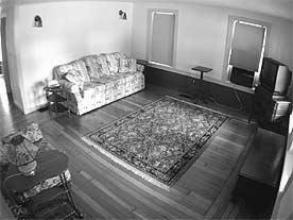
\includegraphics[width=\textwidth]{img/livingroom_hard}
					\caption{Livingroom}
					\label{fig:livingroomhard}
	\end{subfigure}
	\caption{Bedrooms and livingrooms are hard to distinguish and therefore to detect}
	\label{fig:hardimages}
\end{figure}

\begin{figure}%
	\centering
	\begin{subfigure}[b]{0.4\textwidth}
					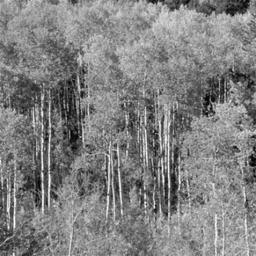
\includegraphics[width=\textwidth]{img/forest_easy}
					\caption{Forest}
					\label{fig:foresteasy}
	\end{subfigure}%
	~ %add desired spacing between images, e. g. ~, \quad, \qquad, \hfill etc.
		%(or a blank line to force the subfigure onto a new line)
	\begin{subfigure}[b]{0.4\textwidth}
					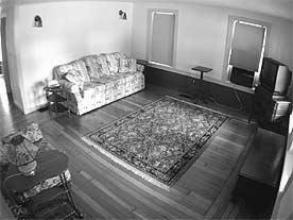
\includegraphics[width=\textwidth]{img/livingroom_hard}
					\caption{Livingroom}
					\label{fig:livingroomeasy}
	\end{subfigure}
	\caption{Forests and livingrooms are easy to distinguish and therefore to detect}
	\label{fig:easyimages}
\end{figure}


\end{document}

% vim:foldmethod=marker
